% Remember to input this to the presentative tex file before compiling.
\chapter{Predicting Pedestrian Trajectories in Driving Environment}

\tab The previous chapter presented an in-depth description and an analysis of the GRIP++ algorithm \cite{li2020gripplus}, explaining its architecture, theoretical foundations, and advantages in predicting trajectories within dynamic traffic environments. To further assess the performance and applicability of GRIP++, the algorithm was implemented on a different dataset from ApolloScape Trajectory dataset \cite{ma2019trafficpredict}, the one originally used by the developers of the algorithm. Instead Joint Attention in Autonomous Driving, (JAAD) \cite{rasouli2017ICCVW} dataset was opted for this operation. JAAD provides extensive examination of joint attention in the autonomous driving context \cite{rasouli2017ICCVW}. The dataset focuses on the behaviour of pedestrians and drivers in a traffic scenario, specifically at the crossing points as well as the factors influencing them. Due to its comprehensive set of annotated videos, it makes it well-suited for the task of predicting pedestrian trajectories and investigating the essential question "Are they going to corss?" \cite{rasouli2017ICCVW}. 

\tab As such this chapter focuses on conversion of JAAD dataset to suitable format, training and testing the dataset to receive predicted trajectory results, which was then incorporated with \verb|YOLO| \cite{yolov3} for object detection and DeepLabV3+ \cite{DBLP:journals/corr/abs-1802-02611} for semantics segmentation to enhance overall accuracy and context-awareness of the predictions. Figure \ref{fig:pipeline} demonstrates the pipeline of this research.

\begin{figure}[h]
  \begin{center}
     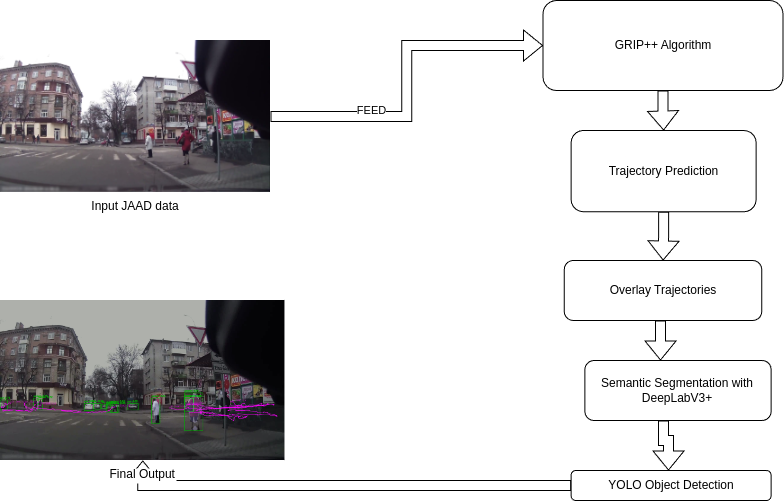
\includegraphics[scale=0.5]{Images/Figures/Pipeline.png}
  \end{center}
  \caption{Pipeline for predicting trajectory in a dynamic driving context}
  \label{fig:pipeline}
\end{figure}

\section{JAAD Dataset}

\tab As briefly mentioned above JAAD provides annotation of a collection of dataset, specially \(346\) short video clips of driving footage, is available to the public for research in autonomous vehicle area. These clips, recorded from various regions of North America and Eastern Europe, capture a variety of common scenes typical of everyday urban driving in a range of weather conditions \cite{rasouli2017ICCVW}. 

\subsection{Annotation Structure of JAAD}

\tab The annotations of JAAD videos are based on the video clip titles. Three kinds of labels are available from JAAD: "pedestrians" (individuals with behavior annotations), "peds" (bystanders who are distant and do not interact with the driver), and "people" (groups of pedestrians) \cite{rasouli2017ICCVW}. The format of each pedestrian's unique id is \verb|0_<video_id>_<pedestrian_number>|. Pedestrians with behavior annotation, have "b" attached at the end of their ids, e.g., \verb|0_1_3b|. Similarly, annotations for people follow the same strucutre but their ids end in the letter "p," such as \verb|0_5_2p|, the annotations for people likewise follow the same structure. For the purpose of using this dataset annotation, however, strings and chars like \verb|"_"|, \verb|"p"|, and \verb|"b"| were removed from the annotations during the \textbf{data transformation} stage since the data structure of the GRIP++ algorithm does not allow for strings to be included in the dataset while preprocessing \cite{ma2019trafficpredict}.

\tab In the annotations, bounding boxes are provided together with occlusion tags for all pedestrians which make the dataset suitable for pedestrian detection. Bounding boxes in each annotation have two coordinate points: the top-left and bottom-right corners, specified as \([x_1, y_1, x_2, y_2]\). Additionally, these bounding boxes are labeled with occlusion tags, where 0 indicates no occlusion, 1 represents partial occlusion (more than 25\%), and 2 denotes full occlusion (more than 75\%).

\tab The annotations within the dataset are categorized into five distinct groups, each for a specific purpose:

\begin{itemize}
    \item \textbf{Annotations}: This group encompasses general video metadata such as attributes related to the time of day, weather conditions, and location. Additionally, it includes detailed information on pedestrian activities (e.g., walking, looking) and bounding box coordinates, along with corresponding occlusion statuses. Notably, activity information is only available for a selected subset of pedestrians. These annotations are recorded for each frame and apply to every labeled instance.
    \item \textbf{Attributes}: Focused on pedestrians with behavior annotations, this category provides demographic details and information regarding crossing points and crossing behavior characteristics. These annotations are assigned to individual pedestrians rather than frames and are intended to offer insights into specific pedestrian behaviors in various traffic scenarios.
    \item \textbf{Appearance}: For videos characterized by high visibility, this group offers details on pedestrian appearance, including pose, clothing, and any objects being carried. This information is annotated per frame for each pedestrian, allowing for a thorough analysis of pedestrian visual characteristics.
    \item \textbf{Traffic}: This group contains traffic-related annotations, offering information on the presence of traffic signs, traffic lights, and other traffic control devices within the scene. These annotations are captured on a per-frame basis, ensuring a comprehensive understanding of the traffic environment during the recorded events.
    \item \textbf{Vehicle}: Vehicle-related actions, such as acceleration, deceleration, or rapid movement, are included in this category and these actions are recorded per frame
\end{itemize}

\tab In the application of the GRIP++ algorithm, not all annotation groups are required. The primary focus is on the dataset annotations group "\textbf{Annotations}," which provide the necessary information for the task. The other groups are considered irrelevant to this particular application and are therefore disregarded.

\section{Data Preparation}

\tab The JAAD dataset, originally structured for analyzing pedestrian behavior in traffic scenarios, required transformation to be suitable with the data format required by the GRIP++ algorithm. The JAAD dataset provides annotations in XML format, detailing pedestrian positions, actions, and interactions with traffic elements. However, the GRIP++ algorithm expects data in a specific structure, similar to the Apolloscape dataset, which was used by the GRIP++ authors for their experiments \cite{li2020gripplus}. To adapt the JAAD dataset to be compatible with GRIP++ requirement, data conversion was carried out. 

\subsection{Data Conversion}

\tab The JAAD dataset contains XML annotations for behavior and interactions of pedestrians in urban environments. These XML annotations were first converted into a structured text format that matches the format used by the Apolloscape dataset. Their data structure of each line in the text file is as follow:

\begin{table}[h!]
\centering
\resizebox{\textwidth}{!}{%
\begin{tabular}{|c|c|c|c|c|c|c|c|c|c|}
\hline
frame\_id & object\_id & object\_type & position\_x & position\_y & position\_z & object\_length & object\_width & object\_height & heading \\
\hline
\end{tabular}%
}
\caption{Data Structure of ApolloScape Dataset \cite{ma2019trafficpredict}}
\end{table}

However, since the JAAD dataset does not include information for position\_z, and object\_height, only eight columns were extracted from the JAAD annotations. These columns include frame\_id, object\_id, object\_type, position\_x, position\_y, and heading. The missing columns (i.e. position\_z and object\_height) were omitted because JAAD lacks the necessary 3D positional information and detailed bounding box dimensions available in Apolloscape.

\subsubsection{Heading Calculation}

\tab Although data for "heading" was not readily available, it was computed based on the already accessible information. The heading is an angular measure that represents the orientation or direction of the object with respect to the x-axis \cite{serway2013physics}. For instance, in a traffic scenario, the heading can indicate whether a vehicle is moving forward, turning, or reversing. 
The heading was calculated based on the position of the object’s bounding box. Specifically, the angle of the vector formed by the top-left and bottom-right corners of the bounding box with respect to the x-axis was computed using the \(atan2\) function. This function calculates the arctangent of the two given coordinates, which provides the angular direction of the bounding box in radians. The formula \cite{atan2_cpp_tutorial} used is:

\begin{equation}
    heading = atan2(y_{br} - y_{tl}, x_{br} - x_{tl}) 
\end{equation}

where (x\_{\text{tl}}, y\_{\text{tl}}) is the top-left corner of the bounding box and (x\_{\text{br}}, y\_{\text{br}}) is the bottom-right corner. This heading value was then rounded to three decimal places for consistency. The heading provided directional information that the GRIP++ model could use to better predict future trajectories of moving objects.

\subsubsection{Object Type Mapping}

\tab Each object in the JAAD dataset was assigned a type based on the classification scheme used in the Apolloscape dataset. The object types in Apolloscape include small vehicles, big vehicles, pedestrians, motorcyclists/bicyclists, and others. These types were mapped to corresponding IDs as follows:

\begin{table}[h!]
\centering
\begin{tabular}{|l|c|c|c|c|c|}
\hline
\textbf{Object Type} & \textbf{Small Vehicles} & \textbf{Big Vehicles} & \textbf{Pedestrian} & \textbf{Motorcyclist and Bicyclist} & \textbf{Others} \\
\hline
\text{ID} & 1 & 2 & 3 & 4 & 5 \\
\hline
\end{tabular}
\caption{ApolloScape's object types and their corresponding IDs \cite{ma2019trafficpredict}}
\label{tab:object_type_ids}  % Label for referencing the table
\end{table}


 since the JAAD dataset primarily focuses on pedestrian behavior and interactions, it does not provide detailed information about other types of objects, such as vehicles or bicyclists. As a result, after converting the JAAD dataset into the required format, only two object types are expected to appear in the processed data:

\begin{itemize}
    \item \textbf{Pedestrians} (ID: 3),
    \item \textbf{Others} (ID: 5)
\end{itemize}


The "Others" category contains any objects that are not classified as pedestrians, though in practice, the JAAD dataset contains very few examples outside of the pedestrian category. The object type mapping was still retained to ensure compatibility with the GRIP++ algorithm, which was designed with the Apolloscape dataset's object type distribution in mind.

\subsection{Data Cleaning}

\tab After converting the JAAD dataset into the required format for use with the GRIP++ algorithm, an additional step of data cleaning was performed. This cleaning process was necessary for ensuring that the data was consistent with the expectations of the GRIP++ model and did not introduce unnecessary noise during training and testing. The key steps involved in this process were as follows:

\begin{enumerate}
    \item \textbf{Handling Missing Values}: During the conversion process, some object annotations may have been incomplete or missing entirely. These instances were identified, and any lines or entries with missing values were either corrected or removed to maintain the integrity of the dataset.
    \item \textbf{Filtering Non-Relevant Objects}: As previously noted, the JAAD dataset primarily focuses on pedestrians, with limited information available for other object types such as vehicles. Object types that did not fit into the defined categories of the GRIP++ model were categorized as "Others" (ID: 5), but were still retained in the dataset for completeness.
    \item \textbf{Removing Empty Files}: During the preprocessing stage, some files were found to be empty, meaning they contained no objects or annotations. These empty files were automatically removed from the dataset since such files provided no valuable information for training or testing.
\end{enumerate}

As a result of this data cleaning process, the dataset was reduced from the originally available \(\textbf{346}\) files to \(\textbf{319}\) files. The removed files either contained no annotations or did not meet the necessary criteria for further processing.

\subsection{Data Splitting}

\tab Once the data was transformed and cleaned, it needed to be divided into training and testing sets to train the model and evaluate its performance. For this purpose, the \verb|train_test_split| function from the \verb|scikit-learn| library was used.

Given the original setup by the GRIP++ developers, where a specific ratio of training to testing data was employed, the same principle was adopted in this implementation. The data was split with a ratio of approximately \(55\) to \(1\), following the precedent set by the authors of the GRIP++ algorithm. This ratio was chosen to maintain consistency with their approach and ensure that the training data was sufficiently large while still allowing for adequate evaluation on the test data.


\section{Training and Testing the Model}

\subsection{Model Training SetUp}

\tab The training of the GRIP++ model was conducted on \verb|Google Colab|, which provides access to NVIDIA GPUs, that is required to run the original \verb|Python| file developed by the authors \cite{li2020gripplus}, ensuring the required computational power and CUDA support necessary for training deep learning models. \verb|Colab| was chosen due to its free availability and built-in shared GPU support, making it suitable for models that require intensive computations like GRIP++.

\verb|PyTorch| was used as the primary framework for implementing and training the GRIP++ model. \verb|PyTorch| provides flexibility and ease of use, particularly for graph-based models, which are integral to GRIP++. The CUDA library was leveraged to ensure GPU acceleration, which speeds up matrix operations, tensor computations, and the backpropagation process during training \cite{cuda2024}.

\subsection{Hyperparameters and Configurations}

\tab Several hyperparameters were set for training the GRIP++ model. These include:

\begin{itemize}
    \item \textbf{Learning Rate}: The learning rate was set to an initial value of 0.01. This value was chosen based on experimentation and previous works, balancing between fast convergence and stability of training.
    \item \textbf{Batch Size}: The batch size was set to 64 for training and 32 for validation. This choice balances memory usage and the stability of gradient updates.
    \item \textbf{Number of Epochs}: The training was conducted for 50 epochs. The original paper experimented with various epochs, and similar values were used here to ensure the model converges appropriately.
    \item \textbf{Optimizer}: The Adam optimizer was selected for its adaptive learning rate capabilities, which are particularly beneficial for models like GRIP++ that have complex architectures and large parameter spaces.
\end{itemize}

These configurations were determined based on the original implementation of GRIP++ and fine-tuning through experimentation to optimize performance on the JAAD dataset.

\subsection{Preprocessing and Data Preparation}


\tab Before training, the transformed dataset underwent preprocessing to ensure it was in the correct format for input into the GRIP++ model. This preprocessing involved:

\begin{itemize}
    \item \textbf{Normalizing Position Data}: The positional data (\verb|position_x| and \verb|position_y|) were normalized based on the maximum values in the dataset to prevent issues related to scale during training.
    \item \textbf{Graph Construction}: Each frame in the sequence was represented as a graph, where objects (e.g., pedestrians, vehicles) were nodes, and the edges represented interactions between them. The features associated with each node included the object's type and its spatial information.
    \item \textbf{Sequence Padding}: The sequences were padded to ensure consistent input dimensions for the GRIP++ model, as deep learning models require fixed input sizes. Shorter sequences were padded, while longer sequences were truncated.
\end{itemize}
    

Once preprocessing was complete, the dataset was ready for the training and testing phases.

\subsection{Training Process}

\tab The training process involved the following steps:

\begin{itemize}
    \item \textbf{\textit{Data Loading:}} The preprocessed dataset was loaded using custom data loaders designed to efficiently batch the data for training and testing. This involved dynamically creating batches of data, including the graphs for each frame sequence and the associated labels.
    \item \textbf{\textit{Forward Pass:}} For each batch, the data was passed through the GRIP++ model, where the graph convolutional layers extracted interaction-aware features, and the LSTM layers predicted future trajectories based on these features.
    \item \textbf{\textit{Backpropagation}}: Gradients were computed using backpropagation, and the Adam optimizer was used to update the model's parameters.
    \item \textbf{\textit{Validation}}: After each epoch, the model was evaluated on the validation set to monitor its performance and adjust the learning rate if necessary.
\end{itemize}

\tab This training cycle was repeated for the specified number of epochs, with model checkpoints saved at intervals to prevent data loss and to enable further fine-tuning if required.

\subsection{Challenges}

\tab During the training process, one of the main challenges encountered was the limitations imposed by the available GPU resources on \verb|Google Colab|. While \verb|Colab| provides access to powerful GPUs, there are restrictions on memory usage and the maximum time for continuous usage. These limitations required careful management of the available resources. Training had to be paused or restarted at times, and model checkpoints were regularly saved to avoid data loss.

\section{Results and Analysis}

\subsection{Model Performance Evaluation}

After training the GRIP++ model on the JAAD dataset, the model's performance was evaluated on the test set. The evaluation focused on predicting the future trajectories of pedestrians, as JAAD primarily contains pedestrian data. The predictions were compared against the ground truth to assess the accuracy of the model.

Key performance metrics included:

\begin{itemize}
    \item Average Displacement Error (ADE): Measures the average Euclidean distance between the predicted trajectories and the ground truth over all time steps \cite{ma2019trafficpredict}. This metric is particularly important in trajectory prediction tasks, as it indicates how close the model's predictions are to the actual movement of the objects.
    \item Final Displacement Error (FDE): Evaluates the distance between the predicted final position and the ground truth final position at the last time step \cite{ma2019trafficpredict}. This metric helps assess how well the model predicts the endpoint of a trajectory, which is critical in safety-critical applications like autonomous driving.
\end{itemize}

\begin{table}[ht]
\centering
\begin{tabular*}{\textwidth}{|c@{\extracolsep{\fill}}|c|c|c|}
\hline
\textbf{Method}            & \textbf{Epoch} & \textbf{ADE} & \textbf{FDE} \\
\hline
TrafficPredict             & -              & 7.1811       & 11.121       \\
\hline
GRIP++            & Epoch18             & 0.7142       & 1.3732       \\
\hline
GRIP++ on JAAD     & Epoch21             & 1.66         & 0.15         \\
\hline
GRIP++ on JAAD     & Epoch41             & 12.26        & 0.57         \\
\hline
\end{tabular*}
\caption{Comparison of methods based on ADE and FDE metrics.}
\end{table}



\tab In the first test subset on the JAAD dataset, the GRIP++ model achieved an ADE of 1.66 and an FDE of 0.15. These results indicate that while the model performs reasonably well in predicting pedestrian trajectories overall, it performed exceptionally in final destination prediction, as evidenced by the relatively low FDE. The low FDE suggests that the model's final predictions were close to the actual final positions of pedestrians in the scene. 

The performance on the second test subset was less accurate, with an ADE of 12.26 and an FDE of 0.57, suggesting that in this scenario, the model struggled more with overall trajectory prediction but still performed relatively better in terms of predicting the final position, though less accurately than in the first test.

\subsection{YOLO and DeepLabV3+}

\tab To get an accurate interpretation of the scene, DeepLabv3+ was employed for semantic segmentation. This deep learning model was used to highlight key features in the driving environment, such as drivable areas and crosswalks. By segmenting the scene, it becomes easier to understand the spatial context within which the pedestrians and vehicles are moving. The segmented output identifies safe zones, walkways, and areas that are off-limits, providing a comprehensive view of how pedestrians interact with their environment. This information is particularly valuable when analyzing whether predicted trajectories falls within safe walking paths or if there is a potential risk of crossing into dangerous areas. The integration of semantic segmentation ensures that trajectory predictions are not only accurate but also contextually aware of the environment.

\tab \verb|YOLO| object detection was used to draw bounding boxes around the objects present in the video frames to keep track of the pedestrians' movements and their interaction in real-time. This helped to distinguish pedestrians from other traffic agents and to associate their predicted trajectory with correct individuals. After the semantics segmentation and YOLO application, predicted trajectories were overlaid on the video frames to depict precisely the movements, ids and the anticipated locations of the pedestrians.  

\tab The visualizations showed how the model predicted the next 3 seconds of pedestrian movement. For instance, the model correctly predicted when a pedestrian was likely to stop, move forward, or change direction. This visual validation was essential to verify the model's effectiveness beyond numerical metrics.




\begin{figure}[h]
  \begin{center}
     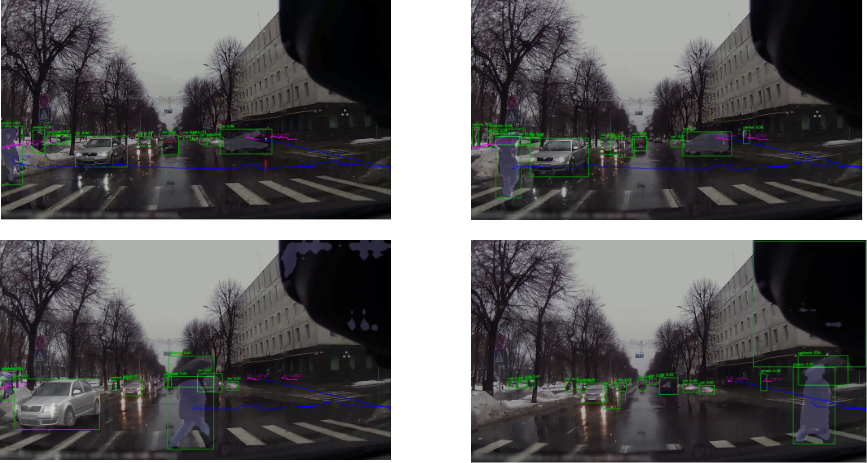
\includegraphics[scale=0.5]{Images/Figures/sequenceofimages.png}
  \end{center}
  \caption{Images from the second test subset}
  \label{fig:testimages}
\end{figure}



\subsection{Qualitative Analysis}

\tab While quantitative metrics like ADE and FDE provide valuable insights, they do not fully capture the complexities of real-world scenarios. One crucial aspect is the inherent uncertainty in pedestrian behavior. Even if the model predicts with 99\% accuracy that a pedestrian will not cross a street, there remains a 1\% chance that they might unexpectedly decide to cross.

\tab This slim margin of uncertainty can have significant consequences. For example, if an autonomous vehicle concludes that a pedestrian is unlikely to cross and continues driving, but the pedestrian suddenly steps into the street, the outcome could be disastrous. Therefore, even models with high predictive accuracy should be used cautiously in critical real-world applications like autonomous driving. Human behavior is unpredictable, and safety systems must account for these rare but potentially catastrophic deviations.

\tab The challenge lies in striking a balance between the model's confidence and the implementation of safety measures that prevent accidents even in rare cases of prediction failure.

\subsection{Challenges and Limitations}


\tab One of the primary challenges encountered during this project was the need for substantial computational resources. The GRIP++ model relies heavily on graph-based computations, which can be resource-intensive. High-performance GPUs and CUDA-enabled environments were essential for training the model efficiently. However, this requirement poses challenges for deploying such models in real-world systems, especially in environments with limited computational capacity, such as cars for which these algorithms are developed in the first place. Another limitation is the gap between academic algorithms and practical implementations. Many algorithms developed in academic research are tailored for desktop-grade GPUs, which require high computational power. However, real-world autonomous driving systems and Advanced Driver Assistance Systems need to be compatible with embedded systems that operate within the constraints of small devices installed in vehicles.

\tab One other limitation comes from the JAAD dataset, which provides annotations only for pedestrians and does not include other relevant and necessary information for other traffic agents like bikers, cyclists, etc. As the dataset is still relatively smaller \cite{rasouli2017ICCVW}, it may be limited to only a certain type of information.